
\section{Higher-Order Dynamics in CISM}
\label{sc:higher-order-into}

\subsection{Basics}
The main distinction between so-called higher-order models and 0-order (or ``shallow ice") models is that higher-order models attempt a closer approximation to solving the non-linear Stokes equations. In general, this usually means incorporating some approximation of horizontal-stress gradients -- along-flow stretching or compression and across-flow shearing -- in addition to the vertical stress gradients that are accounted for in shallow ice models (Figure \ref{fig:stressbalance}). This is important for several reasons:

\begin{figure}
  \begin{center}
    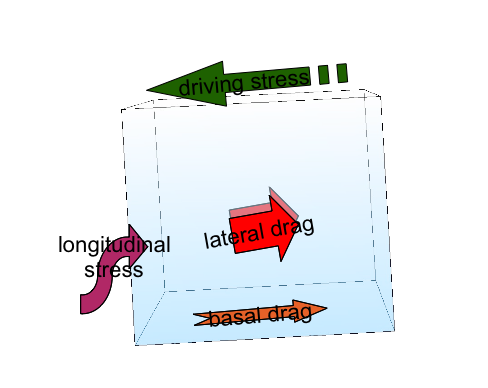
\includegraphics[width=0.5\columnwidth]{\dir/figs/StressBalance.eps}
  \end{center}
  \caption{The gravitational stress available to move the ice is the driving stress, indicated in green. Because the ice is assumed to be in equilibrium, the sum of the other stresses is equal to (i.e., must balance) the gravitational driving stress. In the 0-order model (shallow-ice approximation) the driving stress is assumed to be balanced by basal drag alone. In higher-order models, this restriction is relaxed and the balance of stresses now includes lateral and/or longitudinal stresses. Importantly, because these stresses must be computed based on conditions outside of the local computational cell (the local ice column), this significantly increases the complexity of the model.}
  \label{fig:stressbalance}
\end{figure} 

\begin{itemize}
\item For parts of the ice sheet that we are the most interested in -- e.g. ice streams, ice shelves, and other regions of fast flow -- horizontal-stress gradients are as or more important than vertical stress gradients. To model the flow in these regions accurately, higher-order models are required.

\item The shallow-ice approximation, applied to situations in which there is basal sliding, gives rise to a singularity in the the vertical velocity. Models compute the vertical velocity by integrating incompressibility.
\end{itemize}

\begin{align*}
\frac{\partial w}{\partial z} = -\frac{\partial u}{\partial x}-\frac{\partial v}{\partial y}
\end{align*}

\begin{description}
\item[]	If there is a jump from no-sliding in one grid cell to sliding in the one next to it, the horizontal velocity gradients at the bed will be entirely dependent on the grid spacing; the horizontal gradients (and through incompressibility, the vertical velocity gradient and thus the vertical velocity) will become increasingly large as the grid spacing decreases. Obviously, this is nonsensical and to be avoided.

\end{description}
\begin{itemize}
\item Incomplete knowledge of the stresses near the grounding line, which are often dominated by horizontal rather than vertical stresses, makes it unlikely that shallow ice models will ever be able to accurately simulate grounding line advance and retreat.

\item In some regions of very slow flow, like ice divides, horizontal-stress gradients are important or dominant. Ice cores are often recovered at ice divides and flow modeling is important for interpreting ice core records and using information (such as layer thickness) to infer the past flow history in the region. In order to model that flow correctly, one must include horizontal stresses (At an ice divide the surface slope is \(\sim\)0, in which case vertical stress gradients that drive deformation in 0-order models are also \(\sim\)0. In reality, deformation is not 0 at ice divides, it is simply controlled by horizontal stretching rather than vertical shearing).
\end{itemize}

The term higher-order comes from scaling analyses of the Stokes equations for which a scaling parameter $\lambda=H/L$ -- the ratio of the thickness to the horizontal length scale of interest -- is used to assign importance to the various terms. Shallow ice models retain only terms of order 0 while higher-order models also retain terms of order 1 (and possibly greater) (Figure \ref{fig:hoeqns}). 

\begin{figure}
  \begin{center}
    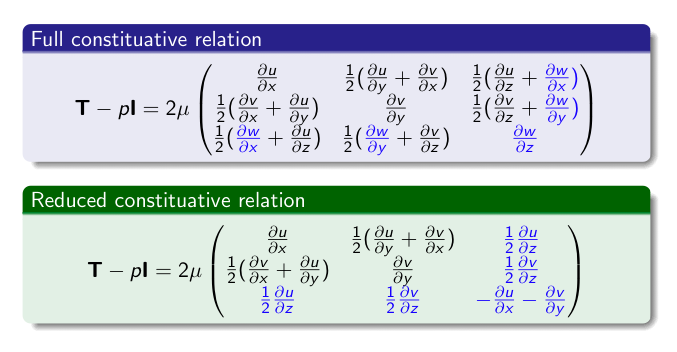
\includegraphics[width=0.7\columnwidth]{\dir/figs/HOeqns.eps}
   \end{center}
  \caption{Stokes-flow (top) and first-order (bottom) constitutive equations.}
  \label{fig:hoeqns}
\end{figure} 

\subsection{Available schemes}

\begin{itemize}
\item The most basic and fundamental higher-order scheme is the full, non-linear Stokes equations. Because of the computational burden, many 3d, large-scale models solve lower-order approximations to the Stokes equations (Figure \ref{fig:phylogeny}). However, a number of groups are making significant advances in this area and it seems likely that 3d, nonlinear-Stokes ice sheet models being used in climate-model applications is not far away (e.g. see the ELMER-Ice effort; \citet{gagliardini:2013iv}). Upcoming DOE-funded efforts will focus on implementing a nonlinear Stokes model on unstructured grids in CISM \citep{Leng:2012ia}.
\end{itemize}

\begin{itemize}
\item Probably the most long-lived higher-order approximation in glaciology is the shallow-shelf approxmation (or SSA) describing flow within an ice shelf (or ice stream if non-zero basal drag is included). It was made popular by Doug MacAyeal in the 80's and 90's (e.g., \citet{Macayeal:1989uo}). It's main disadvantage is that it is not fully 3d, as it assumes uniform velocity throughout the ice thickness driven only by horizontal stress gradients. It is, however, adequate for describing fast flow in many parts of the ice sheets, such as on ice shelves and along some ice streams. In this case, not resolving vertical gradients is a computational advantage.   
\end{itemize}

\begin{itemize}
\item The SSA equations are actually a depth-averaged form of a more general higher-order model, which is commonly referred to as the ``Blatter-Pattyn model" (\citet{BLATTER:1995wz}; \citet{Pattyn:2003tj}). This model has been around since the mid 90's and has become increasingly popular ever since. Blatter-Pattyn dynamics, synonymous with and more formally described as the ``first-order accurate Stokes approximation"\footnote{See \citet{Schoof:2010dl} and \citet{DUKOWICZ:2010wb} for a more complete scaling analysis and derivation of the first-order Stokes approximation.}, are currently implemented as the default higher-order dynamical core within CISM. 
\end{itemize}

\begin{itemize}
\item Several hybrid schemes exist that are computationally cheaper than the Blatter-Pattyn model. These combine solutions to the shallow ice approximation (for resolving vertical gradients) and the SSA approximation (for resolving horizontal gradients) in some clever way so that a fully 3d solution is obtained. It isn't yet known how well these model solutions compare to fully 3d models, or if one approach (hybrid vs. fully 3d solution) is superior to the other. David Pollard of Penn State and Ed Bueler of Univ. of Alaska Fairbanks currently run large-scale implementations of this type of model (\citet{Bueler:2009ee}; \citet{Pollard:2009ed}).
\end{itemize}

A good review paper that goes into a fair amount of detail about the various ice flow modeling approximations, their derivations, and their applicability, is the recent review by \citet{Schoof:2013is}.

\subsection{Shallow-ice vs. higher-order models: practical differences}

\begin{figure}
  \begin{center}
    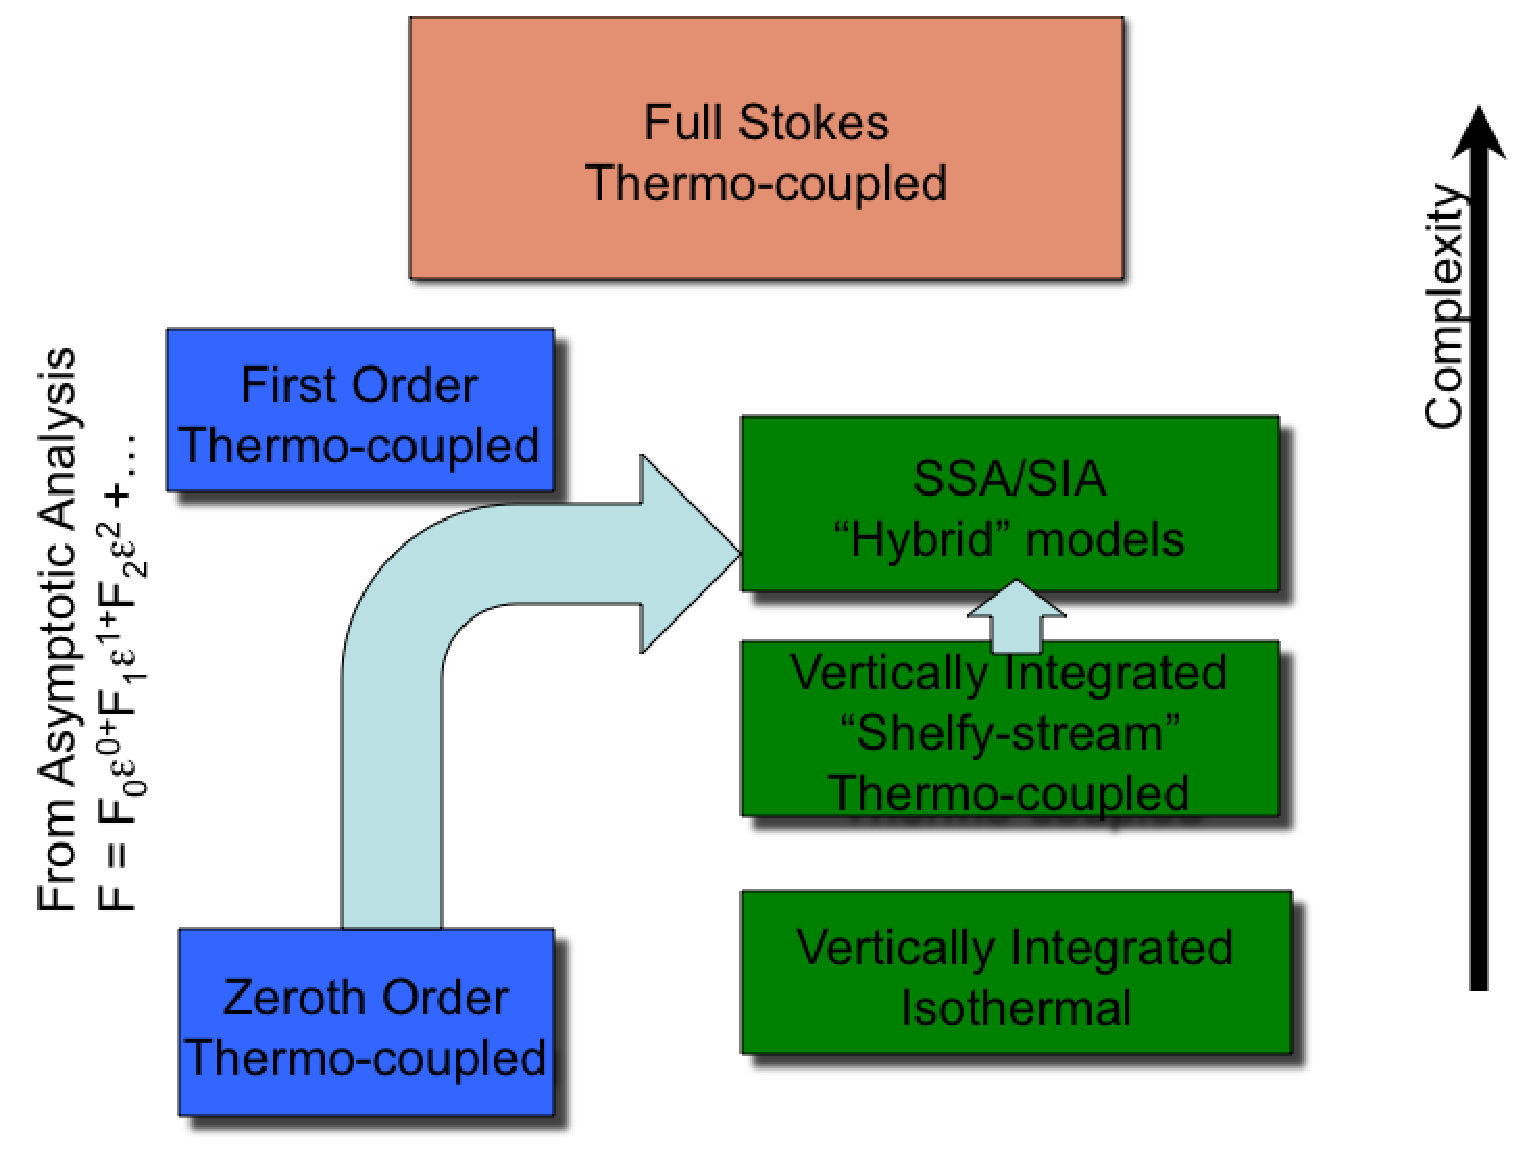
\includegraphics[width=0.5\columnwidth]{\dir/figs/ISMPhylogeny.eps}
   \end{center}
  \caption{The relationship between several common varieties of ice sheet modesl. Complexity increases along the vertical axis.}
   \label{fig:phylogeny}
\end{figure} 

Here, by practical differences, we mean \textbf{(1)} how do we deal with solving the momentum equations (the dynamics, or stress balance) in each case and \textbf{(2)} how do we use the relevant information we derive from that solution (the kinematics, or velocity fields) to evolve the ice sheet geometry in time? There are large differences in how both of these issues are handled -- in shallow ice models versus in higher-order models -- for two main reasons:

\begin{itemize}
\item  The numerical solution of the dynamical equations is fundamentally different in each case. For the shallow ice case, we need only local information (slope and thickness) to solve for the velocity as a function of depth in a single column of ice. We do this pointwise for every location on our model domain (in map view), which is a relatively easy numerical problem; each column of velocities leads to a banded coefficient matrix that is easy to invert (to solve for the velocities). This problem is also what we might call $embarrassingly$ $parallel$; in theory, each column of unknown velocities results in its own tridiagonal matrix, which could be solved for on its own processor. For higher-order models, however, we cannot do this since the solution at any point also depends on the solution at neighboring points (in map plane). The velocity at any point depends on non-local information, leading to an elliptic system of equations, and every velocity must be solved for simultaneously with every other velocity. The result is a much larger system of equations to solve, which is a more difficult numerical problem to solve on one processor and a much more difficult problem to solve on multiple processors. Because large-scale applications of higher-order models (e.g. whole-ice sheet models and coupling with climate models) will require efficient, robust solution and parallelization techniques, this is a very active area of current research.  
\end{itemize}

\begin{itemize}
\item  The equations governing dynamics AND evolution in a shallow-ice model can be recast together as a single, non-linear, diffusion equation for ice thickness. A single system of equations is solved to calculate the velocity field and evolve the ice sheet geometry. For higher-order models, we must first solve the momentum balance equations to obtain the velocity field. Then, we need to use some other scheme to evolve the ice thickness. 
\end{itemize}

Both of these differences mean that a model based on shallow ice physics may be built in a fundamentally different way than one based on higher-order physics. Most of the development work on CISM during the past few years has had to do with upgrading the model so that it can be used effectively and efficiently with higher-order dynamics schemes.  

%The equations describing a (2d) higher-order flow that is vertically integrated (i.e., the SSA) are:
%
%\begin{align*}
%\frac{\partial}{\partial x}\left ( 2 \eta H 
%\left(2\frac{\partial u}{\partial x}+\frac{\partial v}{\partial y}\right)\right)
%+\frac{\partial}{\partial y}\left(\eta H\left(
%\frac{\partial u}{\partial y}+\frac{\partial v}{\partial x}\right)\right)
%=\rho_w gH \frac{\partial s}{\partial x}
%\end{align*}
%
%
%\begin{align*}
%\frac{\partial}{\partial y}\left ( 2 \eta H 
%\left(2\frac{\partial v}{\partial y}+\frac{\partial u}{\partial x}\right)\right)
%+\frac{\partial}{\partial x}\left(\eta H\left(
%\frac{\partial u}{\partial y}+\frac{\partial v}{\partial x}\right)\right)
%=\rho_w gH \frac{\partial s}{\partial y}
%\end{align*}

The equations describing a (3d) higher-order\footnote{Specifically, the first-order accurate Stokes approximation discussed above. These will be derived in more detail in Section \ref{sc:higher-order-mom}.} flow are:

\begin{align*}
  & x: \frac{\partial}{\partial x}\left ( 2 \eta  
\left(2\frac{\partial u}{\partial x}+\frac{\partial v}{\partial y}\right)\right)
+\frac{\partial}{\partial y}\left(\eta \left(
\frac{\partial u}{\partial y}+\frac{\partial v}{\partial x}\right)\right)
+\frac{\partial}{\partial z}\left(\eta \frac{\partial u}{\partial z}\right)
=\rho_w g \frac{\partial s}{\partial x}
\end{align*}


\begin{align*}
  & y: \frac{\partial}{\partial y}\left ( 2 \eta 
\left(2\frac{\partial v}{\partial y}+\frac{\partial u}{\partial x}\right)\right)
+\frac{\partial}{\partial x}\left(\eta \left(
\frac{\partial u}{\partial y}+\frac{\partial v}{\partial x}\right)\right)
+\frac{\partial}{\partial z}\left(\eta \frac{\partial v}{\partial z}\right)
=\rho_w g \frac{\partial s}{\partial y}
\end{align*}

%There are three differences that you should note
Based on these equations, we can point out a few of the important differences between shallow-ice and higher-order models: 
\begin{enumerate}
%\item  The vertically integrated model includes the ice thickness, $H$, in each term. This is a reflection of the integration and does not appear in the first-order equations.
%\item  Accounting for the thickness not appearing, the only other difference is the presence of a vertical diffusion of horizontal velocities. This is the the third term on the left in the above equations.
\item  The the third term on the left-hand side represents the vertical diffusion of horizontal velocities. In a shallow-ice model, this term alone accounts for all ice dynamics and balances the entire body force in the $x$ direction (the term on the right-hand side). Note that the velocity gradients are in the vertical \textit{only}, which is why the solution is ``local" (in map view).

\item  The first-order equations must be solved for each of a set of horizontal layers (the number of which is defined by the resolution in the vertical, here $dz$). These layers communicate with each other through the vertical diffusion term.

\item  The first and second sets of terms on the left-hand side represent the resistance to the body-force term that result from ``membrane stresses". That is, stresses arising from horizontal velocity gradients. It is these horizontal gradients that make this a ``non-local" (elliptic) problem.

\item  The lack of these membrane stress terms in the shallow-ice momentum balance is the primary reason for their failure to realistically simulate the flow in the parts of ice sheets we are most interested in -- outlet glaciers, ice streams, and ice shelves -- where horizontal stress gradients are not small, or may even be the dominant terms.  

\end{enumerate}

%Both sets of equations are non-linear elliptical equations and much of the same technology can be used solve them. 
Additional complications come in when we account for boundary conditions at the lateral margins of the domain and at the upper and lower surfaces of the flow. We describe both the governing equations above and these boundary conditions in more detail in the sections below.
% (note that for the vertically integrated flow, there are no explicit boundary conditions for the upper and lower surfaces; they are accounted for and incorporated during the vertical integration).

%\subsection{Higher-order CISM}

%A very useful higher-order model intercomparison project (ISMIP-HOM) was organized by Frank Pattyn from the Université Libre de Bruxelles. That project, which resulted in a set of "benchmark" experiments for higher-order models, is reported on formally in Pattyn et al. (2008). 
